\documentclass{article}
\usepackage{amsmath}
\usepackage{fullpage}
\usepackage[dvips]{graphicx}


\newcommand{\DO}{\mbox{D\O}}
\newcommand{\Bs}{\mbox{$B_{s}^{0}$}}
\newcommand{\Bsbar}{\mbox{$\bar{B_{s}^{0}}$}}
\newcommand{\Tag}{\mbox{\tt tag}}
\newcommand{\erf}{\mbox{erf}}


\begin{document}

\title{\bf \Bs-\Bsbar\ Mixing Limits Note}

\author{Jamie E. Hegarty and  Phil Gutierrez}

\maketitle


%%%%%%%%%%%%%%%%%%%%%%%%%%%%%%%%%%%%%%%%%%%%%%%%%%%%%%%%%%%%%%%%%%%%%%%%%%%%
\begin{center}
Using an unbinned likelihood amplitude fitting method with a toy Monte Carlo simulation of \mbox{\Bs-\Bsbar} mixing events, we have determined preliminary sensitivity values for a measurement of dilution.
\end{center}


%%%%%%%%%%%%%%%%%%%%%%%%%%%%%%%%%%%%%%%%%%%%%%%%%%%%%%%%%%%%%%%%%%%%%%%%%%%%
\section{The Math}

The lifetime distributions of the mixed ($M$) and unmixed ($U$) states are given by:
\begin{displaymath}
	U(t) = e^{-\frac{t}{\tau}}[ 1 + \cos (\Delta m t) ], 
	\quad \mbox{and} \quad 
%	\,\,\mbox{\hspace{0.25in}and\hspace{0.25in}}\,\,
	M(t) = e^{-\frac{t}{\tau}}[ 1 - \cos (\Delta m t) ]
	\quad \Rightarrow \quad 
	%\end{displaymath}
	%\begin{displaymath}
%	\mbox{such that}\,\,
	\frac{U(t)-M(t)}{U(t)+M(t)} = \cos(\Delta m t) 
\end{displaymath}
where $\tau$ is the mean lifetime of the \Bs.  With mistagging included, the distributions of mixed ($N_{m}(t)$) and unmixed ($N_{u}(t)$) \Bs\ become:
\begin{eqnarray*}
	N_{m}(t) = (1-\alpha)M(t) + \alpha U(t) 
	= (1-\alpha)\{e^{-\frac{t}{\tau}}[1-\cos(\Delta m t)]\} 
	+ \alpha\{e^{-\frac{t}{\tau}}[1+\cos(\Delta m t)]\}
	\\
	N_{u}(t) = (1-\alpha)U(t) + \alpha M(t) 
	= (1-\alpha)\{e^{-\frac{t}{\tau}}[1+\cos(\Delta m t)]\} 
	+ \alpha\{e^{-\frac{t}{\tau}}[1-\cos(\Delta m t)]\}
\end{eqnarray*}
where $\alpha$ is the mistag rate, and dilution $D$ is defined as $1-2\alpha$.
Since $N_{m}(t)$ and $N_{u}(t)$ differ by only the sign of the $\cos(\Delta m t)$ terms, an extra paramter ``\Tag" may be used, such that $\Tag\ =1$ corresponds to the mixed stated, and  $\Tag\ =-1$ corresponds to the unmixed state. The separate $N_{m}(t)$ and $N_{u}(t)$ can be generalized to a single distribution function:
\begin{equation}
        N(t,\Tag) = (1-\alpha)\{e^{-\frac{t}{\tau}}[ 1 -\Tag\cdot \cos(\Delta m t) ]\} 
	+ \alpha\{e^{-\frac{t}{\tau}}[ 1 + \Tag\cdot \cos (\Delta m t) ]\}
\end{equation}
However, Gaussian smearing to account for the time resolution of the detector must also be factored in. The time-smeared distributions of the mixed and unmixed \Bs\ are found by convoluting $N(t,\Tag)$ with the (normalized) Gaussian $G(t)=\frac{1}{\sqrt{2\pi}\,\sigma}e^{-(\frac{t}{\sqrt{2}\sigma})^2}$:
\begin{displaymath}
        f(t,\Tag) = 
	 \frac{(1-\alpha)}{\sqrt{2\pi}\,\sigma}
	 \int_{-\infty}^{\infty}e^{-(\frac{t-t'}{\sqrt{2}\sigma})^2}
	e^{-\frac{t'}{\tau}}[ 1 -\Tag\cdot \cos(\Delta m t')]\,\,dt\,\,	\ldots
\end{displaymath}
\begin{displaymath}
	\mbox{\hspace{2in}} \,\, + \frac{\alpha}{\sqrt{2\pi}\,\sigma}
	\int_{-\infty}^{\infty}e^{-(\frac{t-t'}{\sqrt{2}\sigma})^2}
	e^{-\frac{t'}{\tau}}[ 1 +\Tag\cdot \cos(\Delta m t')]\,\,dt 
\end{displaymath}
Integrating and making a few simplifying substitutions yields a function suitable to fit with:
\begin{equation}
\label{fitfunc}
	f(t,\Tag) = (1-2\alpha)\frac{e^B}{2\tau}\left[1+\erf(A)-\mbox{\tt tag}\cdot w_r^-e^{-A^2}\right] 
		+ \alpha\frac{e^B}{2\tau}\left[1+\erf(A)+\mbox{\tt tag}\cdot w_r^-e^{-A^2}\right]
\end{equation}
\[	 
	A=\frac{t}{\sqrt{2}\,\sigma}-\frac{\sigma}{\sqrt{2}\,\tau}\,\,; \mbox{\hspace{0.5in}} 
	B=\frac{\sigma^2}{2\tau^2}-\frac{t}{\tau}\,\,; \mbox{\hspace{0.5in}} 
	C=\frac{\sigma \Delta m}{\sqrt{2}}
\]

\noindent where $w_r^-$ is the real part of the complex error function $w(z)$~\cite{cwerf}, evaluated at $z = C - iA$. It is important to note that as $A$ increases, the term $w_r^-e^{-A^2} \rightarrow \cos(2AC)$.\\

%%%%%%%%%%%%%%%%%%%%%%%%%%%%%%%%%%%%%%%%%%%%%%%%%%%%%%%%%%%%%%%%%%%%%%%%%%%%
\section{Monte Carlo Simulation}

\Bs\ events are generated with Root~\cite{root} using a toy Monte Carlo (MC) simulation, as follows:

\begin{enumerate}
\item For each event, the proper lifetime $t_p$ of the \Bs\ is first selected from a perfect exponential distribution with a mean at $\tau = 1.5 \times 10^{-12}s$. Next, a random time ``smearing'' value, selected from a Gaussian distribution centered at zero, with $\sigma = \sigma_t$, is added to the proper time $t_p$.
This smearing is intended to represent the time-resolution limitations of the detector.  

\item The new, smeared time, is then smeared again with a second Gaussian centered at zero, but having a lifetime-dependent\footnote{We're in the rest frame of the \Bs.} $\sigma = \sigma_nt_p$.  This second smearing is intended to account for unmeasured neutrinos in the decay of the \Bs, which carry away a proportionally larger amount of momentum for long-lifetime \Bs\ than for short-lifetime \Bs, regardless of the decay mode\footnote{This will soon be updated to use a distribution which takes decay mode, among other things, into account.}, thus adding more error to the determination of the decay length of longer-lifetime \Bs.  The final, ``measured'' time, is then $t$.

\item Next, it is decided whether or not the \Bs\ in an event ``mixes'' by comparing a number selected from a flat random distribution between 0 and 2 with the value of $1+\cos(\Delta m t_p)$ (the mixing comparison), where $\Delta m$ is the mass difference between the \Bs\ and \Bsbar.  If the first number is larger than the mixing comparison, the \Bs\ has mixed to a \Bsbar\, otherwise it remains ``unmixed''.  In either case, it is tagged accordingly.

\item Finally, the possibility of mistagging is considered, at a percentage rate\footnote{\label{dilution}The dilution $D = 1-2\alpha$.} $\alpha$.  This is the percentage of events for which a \Bs\ is actually supposed to be a \Bsbar\, or vice versa.  A number is selected from a flat random distribution between 0 and 1, and compared to $\alpha$ to determine whether the particle is mistagged, smaller numbers than $\alpha$ indicating that this is the case.  The tag of the particle is then adjusted accordingly.
\end{enumerate}
To run this simulation, the user must specify:
\begin{table}[h]
\begin{center}
\begin{tabular}{r@{\,\,\,}l@{\hspace{0.25in}}r@{\,\,\,}l@{\hspace{0.25in}}r@{\,\,\,}l@{\hspace{0.25in}}}
	
	{\tt tSigma}: & $\sigma$ for time-independent smearing 
	& {\tt nEvts}: & The number of events 
	& {\tt dm}: & $\Delta m$ \\	
	{\tt nSigma}: & $\sigma$ for time-dependent smearing 
	& {\tt misTag}: & The mistag rate ($\alpha$) 
	& {\tt tau}: & $\tau$  \\

\end{tabular}
\end{center}
\end{table}

\noindent The MC is also currently capable of generating a simple exponential background, with a user-definable signal-background ratio, but we have not used this functionality yet.


%%%%%%%%%%%%%%%%%%%%%%%%%%%%%%%%%%%%%%%%%%%%%%%%%%%%%%%%%%%%%%%%%%%%%%%%%%%%
\section{The Fitting}

Each set of generated events is histogrammed by lifetime, depending on the tag, and fit with a function\footnote{ {\tt mll\_fit\_d()} in {\tt unbinFitosc\_d.cpp.}, which refers to {\tt lftmosc\_plt\_d()} and {\tt mixing()} in {\tt func.cpp} } which takes the following as parameters: $\Delta m$, $\sigma_t$, $\tau$, {\tt tag}, $\alpha$, and $t$, where $t$ is the independent variable.  The actual fit function is given by Equation~\ref{fitfunc}, and uses RooFit~\cite{roofit} for computation of the complex error function.\\

\noindent The code used for fitting ({\tt unbinFitoscd.cpp}) utilizes Root's version of MINUIT~\cite{minuit} to do an unbinned likelihood fit, meaning that generated values of the lifetime $t$ are compared to the distribution function $f$ individually (and therefore independent of any histogram binning), to determine the probability of selecting that value of $t$ from the distribution $f$.  MINUIT adjusts the fit parameter(s) in small steps, and runs the test against $f$ over again until the probability is maximized, and then returns the final value of the fit parameter(s) and the associated error.\\

\noindent By ``fixing'' all parameters but $\alpha$ during the fit, we have essentially fit for only the amplitude of the oscillation, hence the ``unbinned likelihood amplitude'' fitting.

%%%%%%%%%%%%%%%%%%%%%%%%%%%%%%%%%%%%%%%%%%%%%%%%%%%%%%%%%%%%%%%%%%%%%%%%%%%%
\section{Calculating Sensitivity \label{calcsens}}

For each set of conditions tested, we calculated the sensitivity of a measurement of dilution ($D = 1-2\alpha$) to the conditions as follows:

\begin{enumerate}
\item The process of generating events and fitting for the dilution was done 20+ times for each run, each time with $\Delta m=1000$ in the MC, and $\Delta m$ in the fit fixed at a value varied between 0 and $\sim$20 over the course of each run\footnote{Values other than 0-20 were used when needed for reasonable precision.}.
\item The {\em error} in $\alpha$, as reported by MINUIT, was plotted against $\Delta m$. {\em (The dots in Figure~\ref{sample}.)}
\item The equation of a straight line crossing through the dilution error value just below 1, and that just above 1, was determined.{\em (The line in Figure~\ref{sample}.)}
\item The {\em Sensitivity} was then calculated to be the value of $\Delta m$ for which this line crossed 1. {\em (The open circle in Figure~\ref{sample}.)}
\end{enumerate}

\begin{figure}
\begin{center}
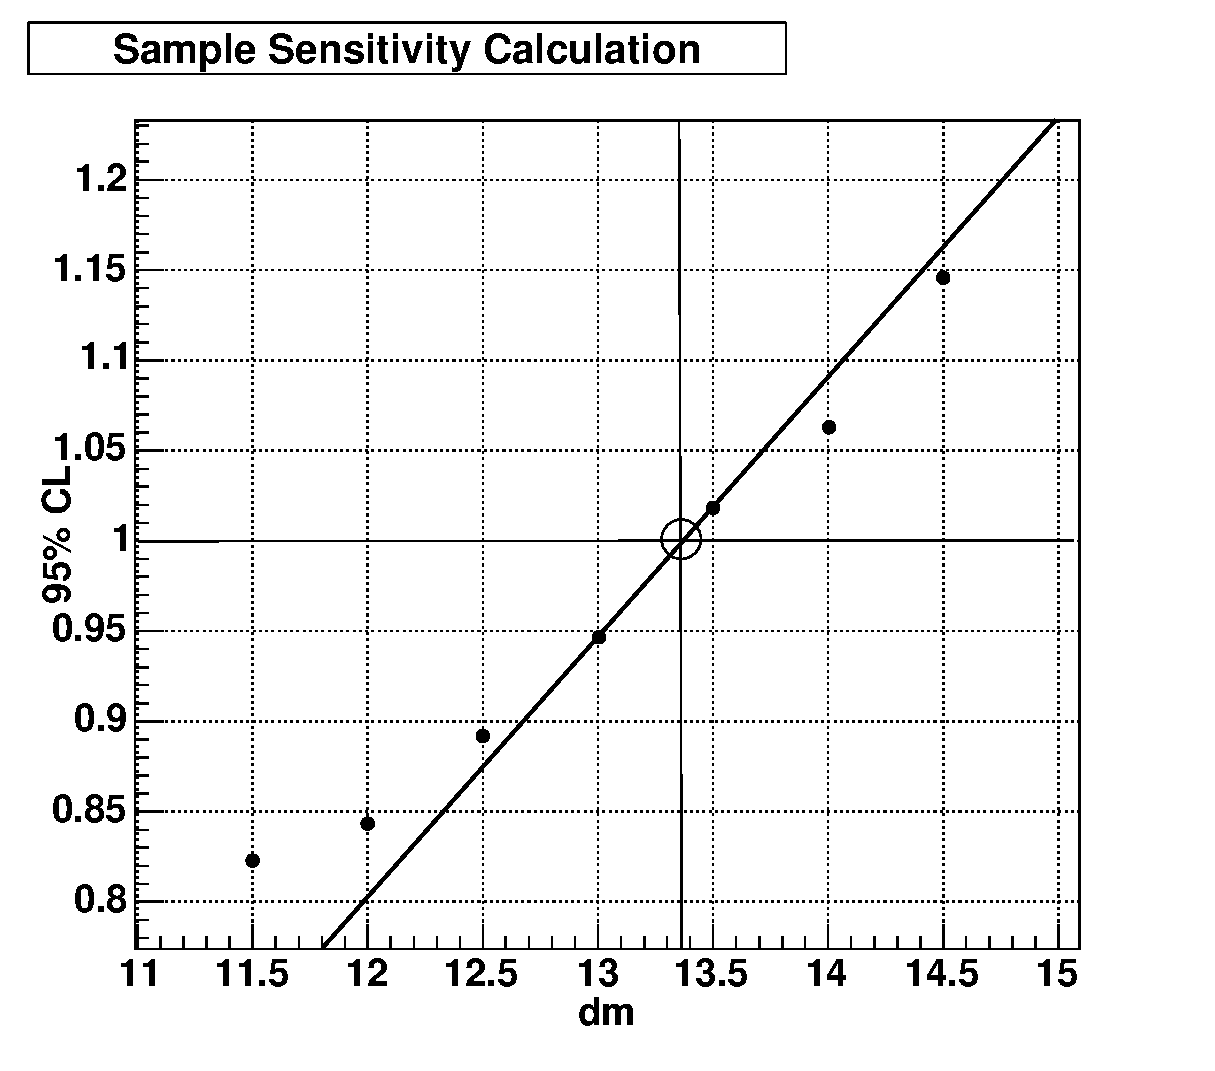
\includegraphics[width=3in]{sample.eps}
\caption{A sample sensitivity calculation.  The sensitivity is defined to be the value of $\Delta m$ for which the error in $D$ is 1. {\em (Dots: Step 1 and 2; Line: Step 3, Cricle: Step 4.)}}
\label{sample}
\end{center}
\end{figure}
\noindent In general, testing the sensitivity of a dilution measurement involved setting one or more parameters differently in the MC than in the fit.

%%%%%%%%%%%%%%%%%%%%%%%%%%%%%%%%%%%%%%%%%%%%%%%%%%%%%%%%%%%%%%%%%%%%%%%%%%%%
\section{Results}

Sensitivity of a dilution measurement was tested under the following conditions:  Variations in $\sigma_t$, variations in $D$, and variations in $\sigma_n$.  In the first two cases, the Condor batch scheduler was used to run the series of tests on the OUHEP cluster~\cite{ouhep}, and in the last case, PBS was used to run the series of tests on OSCER~\cite{oscer}.  Each sensitivity value represents a run of 20 generate-and-fit iterations, with $\Delta m$ varied between 0 and $\sim$20 over the course of the run, as described in Section \ref{calcsens}.

\subsection{Variations in $\sigma_t$}

{\renewcommand{\arraystretch}{1.25}
\begin{table}
\begin{center}
\caption{Sensitivity of $D$ to $\pm$ 20\% variations in $\sigma_t$}
\label{Tts}
\vspace{0.25cm}
\begin{tabular}{|c||@{\hspace{1cm}}c@{\hspace{1cm}}|@{\hspace{1cm}}c@{\hspace{1cm}}|@{\hspace{1cm}}c@{\hspace{1cm}}|}
	\hline\hline
	Fit $\downarrow$ $\backslash$ MC $\rightarrow$ & 0.08 & 0.10 & 0.12 \\
	\hline\hline
	0.08 & 22.07 & 23.56 & - \\
	\hline
	0.10 & 17.66 & 17.74 & 17.88 \\
	\hline
	0.12 & - & 15.74 & 15.00 \\ 
	\hline\hline
\end{tabular}
\end{center}
\end{table}
}

The effect of $\pm$ 20\% variations in $\sigma_t$ on the sensitivity of $D$ are enumerated in Table \ref{Tts}.  Here, the dilution was set to 0.16 both in the MC and as an initial value in the fit, and time-dependent smearing was not used. $\sigma_t$ was set to values of 0.1 $\pm$ 20\% in the MC, and for each of these, fitting was done with $\sigma_t$ values of 0.1 $\pm$ 20\%.  The combinations for which the listed sensitivity is ``-'' were not tested.

\subsection{Variations in $D$}

{\renewcommand{\arraystretch}{1.25}
\begin{table}
\begin{center}
\caption{Sensitivity of $D$ to $\pm$ 20\% variations in $D$}
\label{Td}
\vspace{0.25cm}
\begin{tabular}{|c||@{\hspace{1cm}}c@{\hspace{1cm}}|@{\hspace{1cm}}c@{\hspace{1cm}}|@{\hspace{1cm}}c@{\hspace{1cm}}|}
	\hline\hline
	Fit $\downarrow$ $\backslash$ MC $\rightarrow$ & 0.128 & 0.160 & 0.192 \\
	\hline\hline
	0.128 & 16.35 & 16.35 & - \\
	\hline
	0.160 & 17.75 & 17.74 & 17.75 \\
	\hline
	0.192 & - & 18.90 & 18.91 \\ 
	\hline\hline
\end{tabular}
\end{center}
\end{table}
}

The effect of $\pm$ 20\% variations in the value of $D$ in the MC vs. the initial value of $D$ used in fitting, on the sensitivity of a measurement of $D$, are listed in Table \ref{Td}.  Here, $\sigma_t$ was set to 0.10 both in the MC and in the fit, and time-dependent smearing was not used. $D$ was set to values of 0.16 $\pm$ 20\% in the MC, and for each of these, fitting was done with $D$ at an initial values of 0.16 $\pm$ 20\%.  The combinations for which the listed sensitivity is ``-'' were not tested.

\subsection{Variations in $\sigma_n$}

{\renewcommand{\arraystretch}{1.25}
\begin{table}
\begin{center}
\caption{Sensitivity of $D$ to $\pm$ 20\% variations in $\sigma_n$}
\label{Ttn}
\vspace{0.25cm}
\begin{tabular}{|c||@{\hspace{1cm}}c@{\hspace{1cm}}|@{\hspace{1cm}}c@{\hspace{1cm}}|@{\hspace{1cm}}c@{\hspace{1cm}}|}
	\hline\hline
	Fit $\downarrow$ $\backslash$ MC $\rightarrow$ & 0.130 & 0.163 & 0.196 \\
	\hline\hline
	$\sigma_n$ ignored & 17.799 & 17.783 & 17.808 \\
	\hline
	Avg.($\sigma_n,\sigma_t$) & 6.473 & 5.840 & 5.162 \\
	\hline
	Eff. $\sigma$ at $t$ & - & 13.386 & - \\ 
	\hline\hline
\end{tabular}
\end{center}
\end{table}
}

Table \ref{Ttn} lists sensitivity of a measurement of $D$ to $\pm$ 20\% variations in $\sigma_n$ vs. variations in accounting for $\sigma_n$ in fitting\footnote{$\sigma_{eff} = \sqrt{\sigma_t^2 + (\sigma_n t)^2} = 0.14$ for $\sigma_t=0.10$ and $t = 0.6$, as experimentally determined.}.  Although the MC makes it easy to include the time-dependent smearing $\sigma_n$, this extra Gaussian is not so easily included into the fit function.  Therefore, we chose three methods of accounting for this extra factor in the fitting.  In the first row of Table \ref{Ttn}, the time-dependent smearing is ignored altogether and \mbox{$\sigma_{eff}$ = $\sigma_t$}.  In the second row, the lifetime values from the MC were histogrammed, and then a bin-weighted average was used to determine an effective (average) value of $\sigma$ to use in the fit.  In the last row, the actual effective smearing at each lifetime $t$ was computed during fitting, using $\sigma_n = 0.163$.  In all cases, $\sigma_t$ was set to 0.1 in the MC and fit, and $D$ was set to 0.16 both in the MC and for the initial fit value.

%%%%%%%%%%%%%%%%%%%%%%%%%%%%%%%%%%%%%%%%%%%%%%%%%%%%%%%%%%%%%%%%%%%%%%%%%%%%
%\section{}

%%%%%%%%%%%%%%%%%%%%%%%%%%%%%%%%%%%%%%%%%%%%%%%%%%%%%%%%%%%%%%%%%%%%%%%%%%%%
\begin{thebibliography}{0}

\bibitem{root} The Root Data Analysis Framework, http://root.cern.ch/.
\bibitem{cwerf} CERNLib C335: Complex Error Function, http://wwwasdoc.web.cern.ch/wwwasdoc/shortwrupsdir/c335/top.html.
\bibitem{roofit} The RooFit Toolkit for Data Modeling {\em (Contains a direct C++ translation of CWERF for use with Root)}, http://roofit.sourceforge.net/.
\bibitem{minuit} CERNLib (PackLib) Long Writeup D506: MINUIT Minimization Package, http://wwwasdoc.web.cern.ch/wwwasdoc/WWW/minuit/minmain/minmain.html.
\bibitem{ouhep} Information about the OUHEP cluster: http://www-hep.nhn.ou.edu/d0/grid/.
\bibitem{oscer} OU Supercomputing Center for Education and Research, http://www.oscer.ou.edu/.
%\bibitem{}
\end{thebibliography}

%\newpage
%%%%%%%%%%%%%%%%%%%%%%%%%%%%%%%%%%%%%%%%%%%%%%%%%%%%%%%%%%%%%%%%%%%%%%%%%%%%
%\begin{appendix}
%{\Large \bf \noindent Appendices}
%\section{Citations \label{cites}}
%
%I cited \cite{root} and all I got was this stupid citation.
%\end{appendix}
%%%%%%%%%%%%%%%%%%%%%%%%%%%%%%%%%%%%%%%%%%%%%%%%%%%%%%%%%%%%%%%%%%%%%%%%%%%%


\end{document}
